\section{Gaussian Processes for Regression}
Mathematical solutions such as linear regression are often used to predict unknown values based on similar values. Depending on input data, output accuracy and simplicity, mathematicians are encouraged to use several other methods as well.
Gaussian Process Regression (GPR) is one of the popular methods has been used due to several reasons such as:
\begin{itemize}
\item Very accurate output
\item Less number of variables
\item Learning by experience
\end{itemize}
Correct predictions must be based on the correct assumptions. Even though GPR is  learning from experience, it is not “free form” which means it is not automatically generated\cite{gausreg}. Other techniques, such as “squared exponential”, can be used when the users are unable to do even basic assumptions.
\\\\
It is acceptable to assume that each observation point has data distribution similar to normal distribution. Therefore, it is needed  to calculate the mean value and variance for all predictions.
\begin{figure}[here]
  \centering
      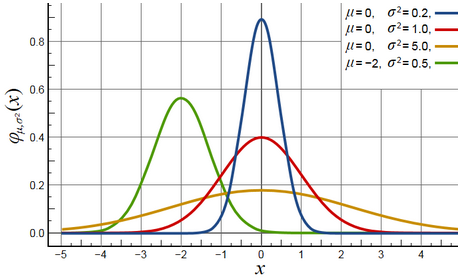
\includegraphics[width=0.9\textwidth]{theory/graphics/normal-distribution.png}
  \caption{Normal Distribution curves\cite{normal-dist}. }
  \label{fig:normal-distribution}
\end{figure}
\subsection{Covariance Function}
In general, users can assume that “partner GP’s mean is zero” everywhere\cite{simple-covariance}. Therefore, two similar cases are related to each other by a covariance function $ k(x-x') $. Among the various options “squared exponential” is one of the popular choices for the covariance function.
\begin{equation}
k(x,x^{'})=\sigma_{f}^{2}exp\left[ \dfrac{-(x-x^{'})^{2}}{2l^{2}} \right]
\label{eq:simple-covariance}
\end{equation}
\begin{eqnarray}
 x - x^{'} &=& Distance\hspace{7pt} between\hspace{7pt} observation\hspace{7pt} data    \nonumber \\
  l &=& length\hspace{7pt} parameter \nonumber \\
  \sigma_{f}^{2} &=& Maximum\hspace{7pt} allowable\hspace{7pt} covariance
\end{eqnarray}
To predict accurate data for a smooth curve, input (or observed) data from the neighbours must be identical. By studying the above equation, it can understood that $ \sigma_{f}^{2} $ is increased for functions which cover a wide area through the y-axis. When the $ (x-x') $value becomes larger, $k(x-x')$ approaches zero depending on the length of parameter $ l $.
\\\\
The effects of the length parameter $l$, can be explained as follows: Lets assume $l=0.1$ for a particular prediction and graph  $f(x)VS x$, which is shown in figure \ref{fig:length-parameter}. It is clear that the curves are not aligned\cite{intro-to-gpr}.
\begin{figure}[here]
  \centering
      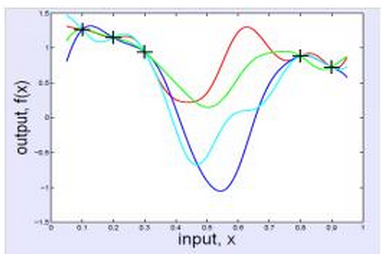
\includegraphics[width=0.65\textwidth]{theory/graphics/effects-of-l.png}
  \caption{When $l = 0.1$. \cite{length-parameter}. }
  \label{fig:length-parameter}
\end{figure}
Then change $l=0.3$ and evaluate the results. This is shown in figure \ref{fig:length-parameter-03}. It is clear that the curves are more aligned here than in figure \ref{fig:length-parameter}.
\begin{figure}[here]
  \centering
      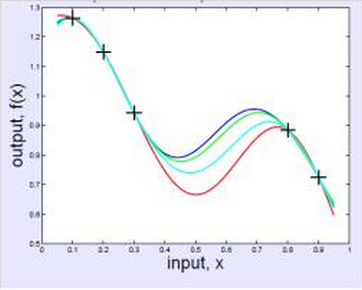
\includegraphics[width=0.65\textwidth]{theory/graphics/effects-of-l-03.png}
  \caption{When $l = 0.3$. \cite{length-parameter}. }
  \label{fig:length-parameter-03}
\end{figure}
Since the curves are not perfectly aligned, length parameter $l$, is increased further and result is evaluated. In figure \ref{fig:length-parameter-05} the $l$ value is set to $0.5$ and evaluate the results. Here one can observe that the curves are perfectly aligned \cite{length-parameter}.
\begin{figure}[here]
  \centering
      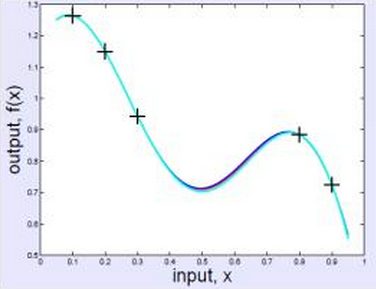
\includegraphics[width=0.65\textwidth]{theory/graphics/effects-of-l-05.png}
  \caption{When $l = 0.5$. \cite{length-parameter}. }
  \label{fig:length-parameter-05}
\end{figure}
Apart from this, function consists of additional part to represent errors. This is an important part, when GPR is used to predict practical events. (e.g. environment temperature can be vary, due to external factors such as wind ).
\begin{equation}
k(x,x^{'})=\sigma_{f}^{2}exp\left[ \dfrac{-(x-x^{'})^{2}}{2l^{2}} \right] + \sigma_{n}^{2}\delta(x,x^{'})
\label{eq:referanceName}
\end{equation}
However, people preferred to keep $ \sigma_{n}^{2} $ separately and work on covariance and error to simplify the calculation.

\subsection{Method of Calculation}
The covariance value, $ k(x,x') $ can be calculated with each observed data in respect to each other observations. Values can be represented by a metric. By assuming that five observations have been conducted, $ x1, x2, x3, x4, x5 $. $k(x,x')$ value for those observations can be written as follows:
\begin{eqnarray}
K = 
\begin{bmatrix} 
k(x_{1}x_{1}) & k(x_{1}x_{2} & k(x_{1}x_{3} & k(x_{1}x_{4} & k(x_{1}x_{5} \\ k(x_{2}x_{1}) & k(x_{2}x_{2} & k(x_{2}x_{3} & k(x_{2}x_{4} & k(x_{2}x_{5} \\
k(x_{3}x_{1}) & k(x_{3}x_{2} & k(x_{3}x_{3} & k(x_{3}x_{4} & k(x_{3}x_{5} \\ k(x_{4}x_{1}) & k(x_{4}x_{2} & k(x_{4}x_{3} & k(x_{4}x_{4} & k(x_{4}x_{5} \\
k(x_{5}x_{1}) & k(x_{5}x_{2} & k(x_{5}x_{3} & k(x_{5}x_{4} & k(x_{5}x_{5} \\ \end{bmatrix}
\label{eq:k-matrix}
\end{eqnarray}

This is a symmetric metric, $k(x1,x2)$ and $k(x2,x1)$  where both elements have the same values. All diagonal elements are equal and show the highest $k(x,x')$ value since $ \dfrac{-(x-x^{'})^{2}}{2l^{2}} $  becomes zero.
\\\\
When the position is moving away from the diagonal line of the matrix, the value of $k(x_{n},x_{m})$ goes towards zero. In other words, if the matrix contain higher number of rows and columns, the values of positions such as far away from the diagonal are almost equal to zero, while diagonal values shows maximum covariance value.
\\\\
While the $K$ matrix gives the covariance values for observed data points the $K*$ matrix gives the covariance values for considered points compared to other observed points. Let’s make the matrix $K_{*}$ relative to the above five positions.
\begin{equation}
K_{*} = [k(x_{*},x_{1}) \hspace{10pt} k(x_{*},x_{2}) \hspace{10pt} k(x_{*},x_{3}) \hspace{10pt} k(x_{*},x_{4}) \hspace{10pt} k(x_{*},x_{5})]
\label{eq:referanceName}
\end{equation}
$K_{**}= k(x_{*} x_{*})$ also can be found same way as it is directly given by $k(x,x')=\sigma_{f}^{2}$. From the above values, mean and variance values for a given $y_{*}$ can be found in the following way:
\begin{eqnarray}
 \overline{y_{*}} &=& K_{*}K^{-1} y    \nonumber \\
 var(y_{*})&=& K_{**}K_{*}K^{-1}K_{*}^{T}
\end{eqnarray}
\begin{eqnarray}
y = 
\begin{bmatrix} 
y_{1} \\ y_{2} \\ y_{3} \\ y_{4} \\ y_{5} \\ \end{bmatrix}
\label{eq:k-matrix}
\end{eqnarray}
When finding the variance, a suitable confidence level must be selected according to the prediction (e.g. 95\% confidence level).
\subsection{Prediction of Values Using Gaussian Process Regression}
The objective is to predict values at a particular point by interpreting other observed data. Imagine the following situation: The area highlighted in gray colour has sensors to observe the values and one would want to predict the value on red colour(3,3) in figure \ref{fig:value-matrix}.
\begin{figure}[here]
  \centering
      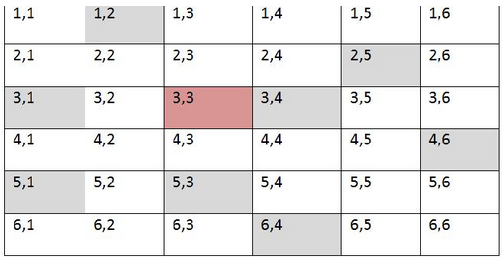
\includegraphics[width=0.65\textwidth]{theory/graphics/value-matrix.png}
  \caption{ Value matrix. }
  \label{fig:value-matrix}
\end{figure}
Since it is possible to find the distance between each cells, it is possible to define a covariance function using observed data (given from sensors). $ \sigma_{f}^{2} $ and $ l $ (length parameter) can be determined by using the observed data. Thereafter, $ K_{**} $, $ K_{*} $, $ K $ matrices can be determined. This will give the values for mean and variance. Finally, it is possible to plot the graph and this will give the predicted values for any positions within the considered area.
